\title{Aula 3 - Conversão de bases}



\begin{frame}
    \titlepage
\end{frame}


\begin{frame}{Conversão de uma base qualquer para base 10}
    Para converter um número de qualquer base $B$ para a base $10$, aplicamos a definição da notação posicional, realizando os cálculos na base 10:

    \begin{block}{Fórmula Única}
        $$ \text{Valor}_{10} = \sum_{i=-k}^{n} b_i B^i $$
    \end{block}

    \begin{itemize}
        \item \textbf{Passo a passo:}
              \begin{enumerate}
                  \item Identifique o peso (potência de $B$) de cada posição.
                  \item Multiplique o dígito pelo seu peso.
                  \item Some todos os resultados.
              \end{enumerate}
    \end{itemize}
\end{frame}

\begin{frame}{Exemplos - Conversão de Binário e Octal para a base 10}
    \begin{itemize}
        \item \textbf{Converver de Binário ($B=2$) para decimal:} $10100,1_2$
              {\small
              $$ (1 \times 2^4) + (0 \times 2^3) + (1 \times 2^2) + (0 \times 2^1) + (0 \times 2^0) + (1 \times 2^{-1}) $$
              $$ 16 + 0 + 4 + 0 + 0 + 0,5 = \mathbf{20,5_{10}} $$
              }

              \vspace{0.4cm}

        \item \textbf{Converver de Octal ($B=8$) para decimal:} $253_8$
              {\small
                      $$ (2 \times 8^2) + (5 \times 8^1) + (3 \times 8^0) $$
                      $$ (2 \times 64) + (5 \times 8) + (3 \times 1) $$
                      $$ 128 + 40 + 3 = \mathbf{171_{10}} $$
                  }
    \end{itemize}
\end{frame}

\begin{frame}{Exemplos de Conversão: Hexadecimal}
    \begin{itemize}
        \item \textbf{Converver de Hexadecimal ($B=16$) para decimal:} $C3_{16}$
    \end{itemize}

    \begin{exampleblock}{Lembrete Importante}
        No sistema hexadecimal, letras devem ser substituídas pelos seus valores decimais antes do cálculo: \textbf{C = 12}.
    \end{exampleblock}

    $$ (C \times 16^1) + (3 \times 16^0) $$
    $$ (12 \times 16) + (3 \times 1) $$
    $$ 192 + 3 = \mathbf{195_{10}} $$
\end{frame}

\begin{frame}{Exercícios: Conversão para Base 10}
    Converta os seguintes números para a base 10, demonstrando a decomposição posicional:

    \begin{enumerate}[a)]
        \item $11011,01_2$
        \item $702_8$
        \item $BF_{16}$
    \end{enumerate}

    \vspace{0.5cm}
    \begin{center}
        \textit{Dica: Comece identificando os expoentes da base a partir da vírgula (para a esquerda $0, 1, 2...$ e para a direita $-1, -2...$).}
    \end{center}
\end{frame}

\begin{frame}{Resposta $11011,01_2$ para decimal}
    \begin{center}
        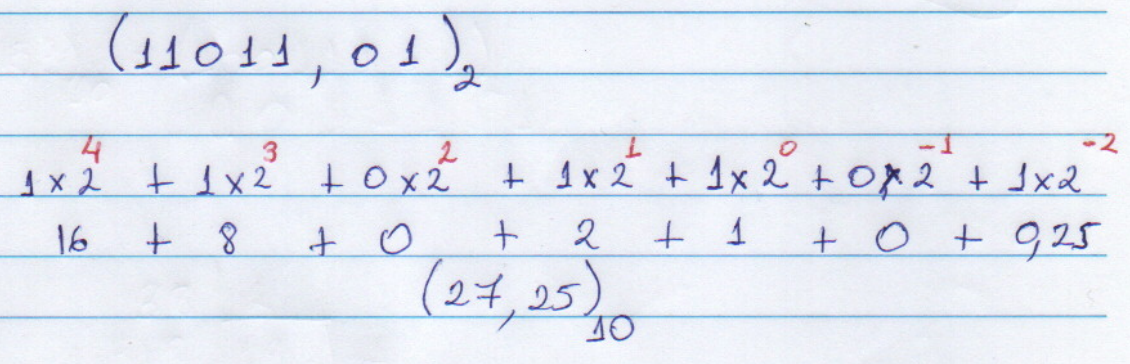
\includegraphics[width=0.9\textwidth]{Figuras/11011-01-to-dec.png}

    \end{center}

    $11011,01_2 = 27,25_{10}$
\end{frame}

\begin{frame}{Resposta $702_8$ para decimal}
    \begin{center}
        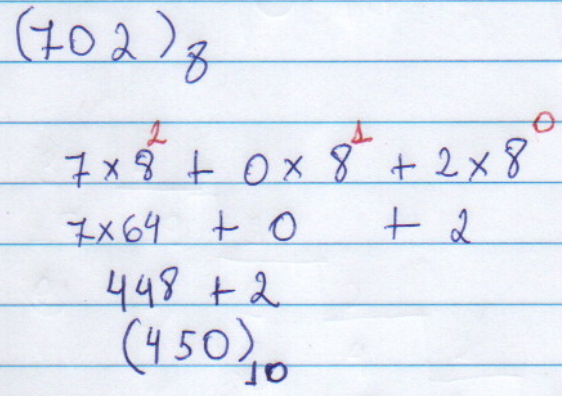
\includegraphics[width=0.9\textwidth]{Figuras/702-to-dec.png}

    \end{center}

    $702_8 = 450_{10}$
\end{frame}

\begin{frame}{Resposta $BF_{16}$ para decimal}
    \begin{center}
        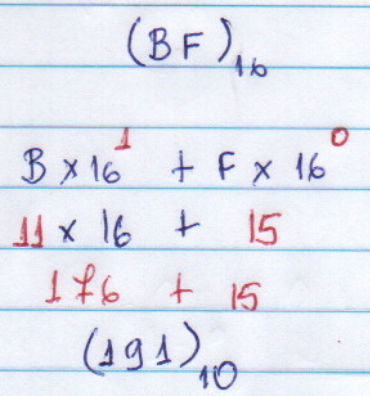
\includegraphics[width=0.5\textwidth]{Figuras/BF-to-dec.png}

    \end{center}

    $BF_{16} = 191_{10}$
\end{frame}

\begin{frame}{Conversão de Decimal para uma base qualquer}
    \begin{itemize}
        \item \textbf{O Método:} Divisões Sucessivas pela base de destino.
        \item \textbf{Propriedade 1:} O resto da primeira divisão é o dígito de menor peso ($b_0$).
        \item \textbf{Propriedade 2:} Ao dividir o quociente sucessivamente, obtemos os dígitos seguintes ($b_1, b_2, \dots$).
        \item \textbf{Encerramento:} O processo termina quando o \textbf{quociente é zero}.
    \end{itemize}

    \begin{block}{Formando o número}
        O resultado é formado pela leitura dos \textbf{restos} na ordem \textbf{inversa} (do último para o primeiro).
    \end{block}
\end{frame}

\begin{frame}{Exemplo Passo a Passo: $9_{10}$ para Binário}
    Vamos converter o número 9 para a base 2:
    \begin{enumerate}
        \item $9 \div 2 = 4$ com \textbf{resto 1} $\rightarrow (b_0)$
        \item $4 \div 2 = 2$ com \textbf{resto 0} $\rightarrow (b_1)$
        \item $2 \div 2 = 1$ com \textbf{resto 0} $\rightarrow (b_2)$
        \item $1 \div 2 = 0$ com \textbf{resto 1} $\rightarrow (b_3)$
    \end{enumerate}

    \begin{exampleblock}{Resultado}
        Lendo os restos do último para o primeiro: $\mathbf{1001_2}$
        $$ 9 = 1 \times 2^3 + 0 \times 2^2 + 0 \times 2^1 + 1 \times 2^0 $$
    \end{exampleblock}
\end{frame}

\begin{frame}{Exemplo do método das divisões sucessivas}
    \begin{center}
        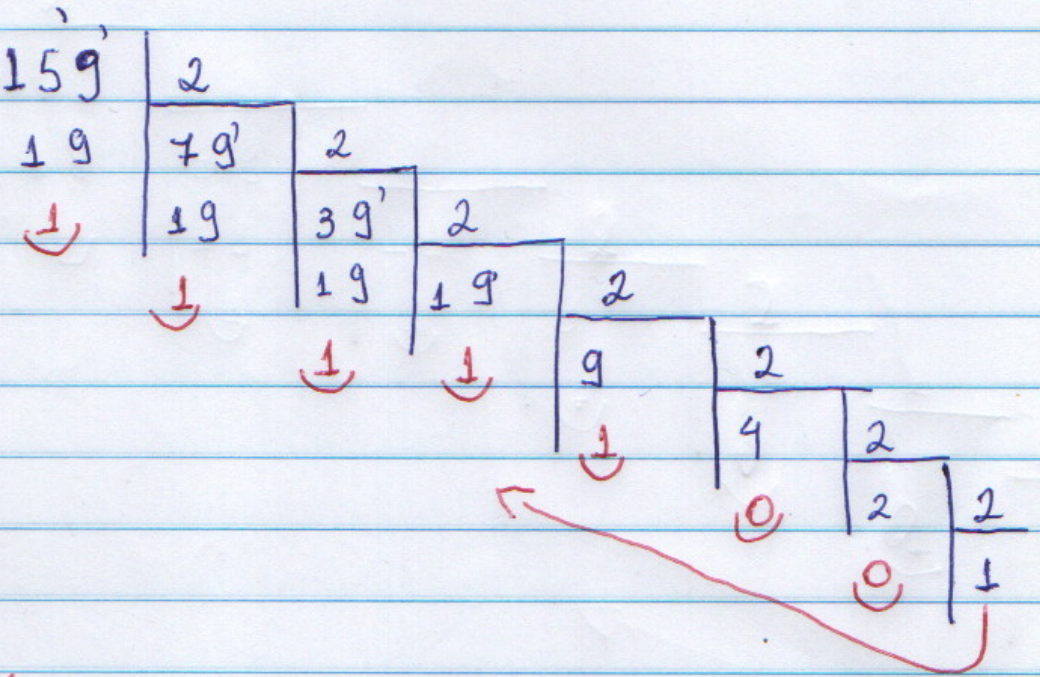
\includegraphics[width=0.7\textwidth]{Figuras/159-to-bin.png}

    \end{center}

    $159_{10} = 10011111_{2}$
\end{frame}

\begin{frame}{Exemplo do método das divisões sucessivas}
    \begin{center}
        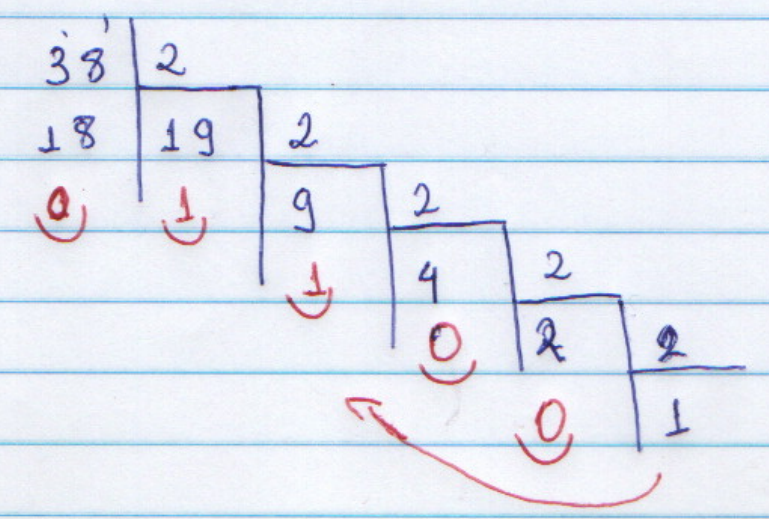
\includegraphics[width=0.7\textwidth]{Figuras/38-to-bin.png}

    \end{center}

    $38_{10} = 100110_{2}$
\end{frame}



\begin{frame}{Conversão: $352_{10}$ para Octal}
    Utilizar uma tabela ajuda a organizar o processo para números maiores:

    \begin{table}[]
        \centering
        \begin{tabular}{|c|c|c|c|c|}
            \hline
            \textbf{Índice} & \textbf{Dividendo} & \textbf{Divisor} & \textbf{Quociente} & \textbf{Resto} \\ \hline
            0               & 352                & 8                & 44                 & \textbf{0}     \\ \hline
            1               & 44                 & 8                & 5                  & \textbf{4}     \\ \hline
            2               & 5                  & 8                & 0                  & \textbf{5}     \\ \hline
        \end{tabular}
    \end{table}

    \begin{itemize}
        \item Lendo os restos de baixo para cima: \textbf{5}, \textbf{4}, \textbf{0}.
        \item \textbf{Resultado:} $352_{10} = 540_8$
    \end{itemize}
\end{frame}

\begin{frame}{Exemplo do método das divisões sucessivas}
    \begin{center}
        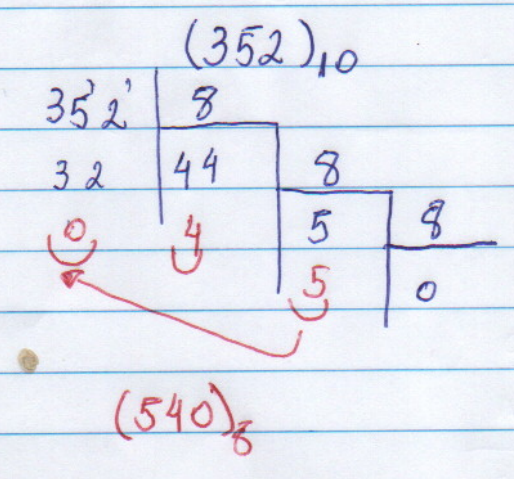
\includegraphics[width=0.7\textwidth]{Figuras/352-to-oct.png}

    \end{center}

    $352_{10} = 540_8$
\end{frame}

\begin{frame}{Conversão de $352_{10}$ para Binário}

    \centering
    \resizebox{\textwidth}{!}{
        \begin{tabular}{|c|c|c|c|c|}
            \hline
            \textbf{Índice} & \textbf{Dividendo} & \textbf{Divisor} & \textbf{Quociente} & \textbf{Resto} \\ \hline
            0               & 352                & 2                & 176                & \textbf{0}     \\ \hline
            1               & 176                & 2                & 88                 & \textbf{0}     \\ \hline
            2               & 88                 & 2                & 44                 & \textbf{0}     \\ \hline
            3               & 44                 & 2                & 22                 & \textbf{0}     \\ \hline
            4               & 22                 & 2                & 11                 & \textbf{0}     \\ \hline
            5               & 11                 & 2                & 5                  & \textbf{1}     \\ \hline
            6               & 5                  & 2                & 2                  & \textbf{1}     \\ \hline
            7               & 2                  & 2                & 1                  & \textbf{0}     \\ \hline
            8               & 1                  & 2                & 0                  & \textbf{1}     \\ \hline
        \end{tabular}
    }
    \\

    Lendo os restos do índice 8 ao 0:
    $101100000_2$


\end{frame}

\begin{frame}{Exercício}

    Escreva sua \textbf{idade} e o \textbf{ano atual} nas seguintes bases, utilizando o método das divisões sucessivas:

    \begin{enumerate}[a)]
        \item Base 11
        \item Base 2
        \item Base 8
        \item Base 16
    \end{enumerate}


\end{frame}

\begin{frame}{Casos especiais onde uma base é potência da outra}



    \begin{itemize}
        \item Para converter de uma base para outra qualquer, sempre é possível
              converter para a base 10 e em seguida da
              base 10 para a base final.

        \item No entanto, em alguns casos (quando uma base é uma potência da outra)
              pode-se evitar esse trabalho.

        \item As técnicas para as bases mais usadas em computação (2, 8 e 16) são exemplificadas a seguir.
    \end{itemize}




\end{frame}

\begin{frame}{Conversão de números em base 8 para base 2}


    \begin{itemize}
        \item A base octal (8) é uma potência da base binária (2): $8 = 2^3$.
        \item Isso permite uma conversão direta e simplificada.
        \item Vamos desenvolver o raciocínio por trás do método.
    \end{itemize}

\end{frame}

\begin{frame}{Passo 1: Expansão posicional - Reescrevendo na base 2}


    Considere o número $253_8$:

    \begin{align*}
        253_8 & = 3 \times 8^0 + 5 \times 8^1 + 2 \times 8^2                                    \\
              & = 3 \times (2^3)^0 + 5 \times (2^3)^1 + 2 \times (2^3)^2                        \\
              & = 3 \times 2^{(3 \times 0)} + 5 \times 2^{3 \times 1} + 2 \times 2^{3 \times 2} \\
              & = 3 \times 2^0 + 5 \times 2^{3} + 2 \times 2^{6}
    \end{align*}

\end{frame}

\begin{frame}{Passo 2: Tentativa inicial}


    \begin{itemize}
        \item Temos os coeficientes $3$, $5$ e $2$ multiplicando potências de $2$.
        \item Seria tentador escrever $2005003_2$, colocando cada dígito em sua posição (0, 3 e 6).

        \item \textbf{Problema:} $2$, $5$ e $3$ \textbf{não são dígitos válidos} na base binária (que só aceita $0$ e $1$).
        \item Precisamos traduzir esses valores ($3$, $5$ e $2$) para sua representação binária.
    \end{itemize}


    \textbf{ATENÇÃO}, nessa hora tome cuidado com mistura de bases

\end{frame}

\begin{frame}{Passo 3: Decomposição dos coeficientes}
    \emph{Transformando $3$, $5$ e $2$ em somas de potências de 2}

    \begin{align*}
        3 & = 1 + 2 =  1 \times 2^0 + 1 \times 2^1 \\
        5 & = 1 + 4 =  1 \times 2^0 + 1 \times 2^2 \\
        2 & = 0 + 2 =  1 \times 2^1
    \end{align*}

\end{frame}

\begin{frame}{Passo 4: Substituição e desenvolvimento}


    \begin{align*}
        253_8 & =  3 \times 2^0 + 5 \times 2^{3} + 2 \times 2^{6}     \\
              & = (1 \times 2^0 + 1 \times 2^1) \times 2^0 \; +       \\
              & \quad (1 \times 2^0 + 1 \times 2^2) \times 2^{3} \; + \\
              & \quad (1 \times 2^1) \times 2^{6}
    \end{align*}

\end{frame}

\begin{frame}{Passo 5: Simplificação}


    Distribuindo e somando os expoentes:

    \begin{align*}
        253_8 & = (1 \times 2^{0}) + (1 \times 2^{1}) \; +     \\
              & \quad (1 \times 2^{3}) + (1 \times 2^{5}) \; + \\
              & \quad (1 \times 2^{7})                         \\[0.5cm]
              & = 2^0 + 2^1 + 2^3 + 2^5 + 2^7
    \end{align*}

\end{frame}

\begin{frame}{Passo 6: O número binário resultante}


    A soma das potências de 2 nos dá a representação binária final:

    \[
        2^0 + 2^1 + 2^3 + 2^5 + 2^7 = 10101011_2
    \]

    Ou seja, $253_8 = 10101011_2$.

\end{frame}

\begin{frame}{Passo-a-passo feito a mão}
    \begin{center}
        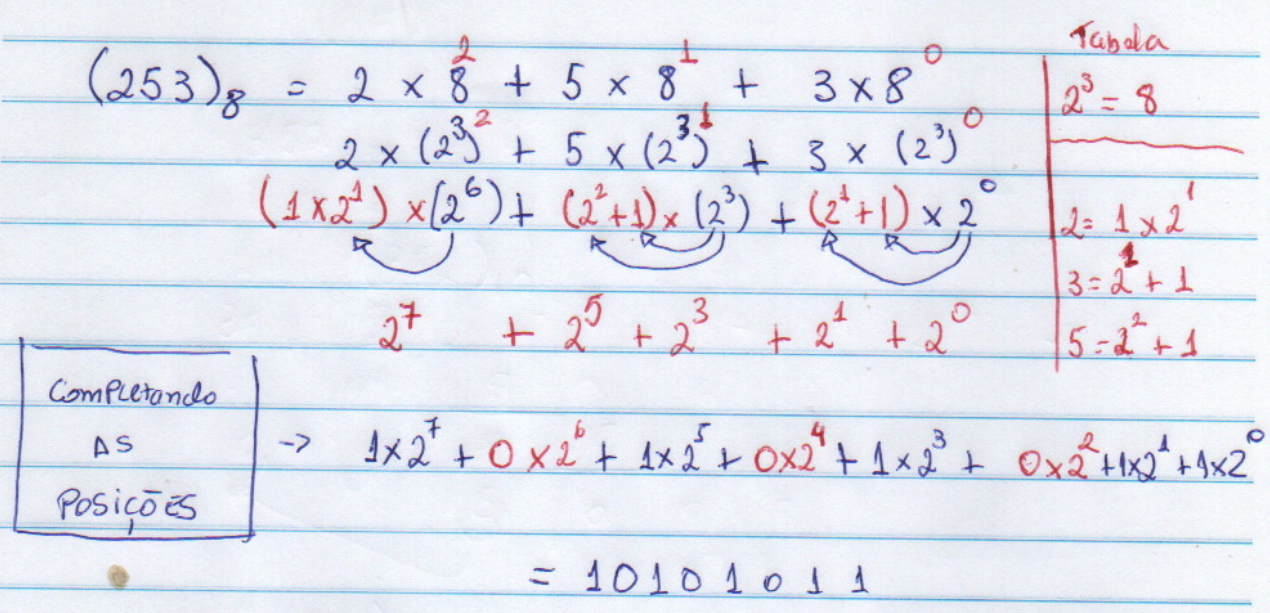
\includegraphics[width=\textwidth]{Figuras/conversao-direta-metodo.png}

    \end{center}


\end{frame}

\begin{frame}{Consequência do resultado anterior}


    O desenvolvimento anterior justifica o método que vamos realmente aplicar:

    \begin{block}{Como fazer?}
        Cada símbolo da representação \textbf{octal} deve ser expandido em sua representação com \textbf{3 bits}.
    \end{block}

    \begin{itemize}
        \item Devem-se usar \textbf{zeros à esquerda} para completar os 3 bits em símbolos menores que 4 ($100_2$).
    \end{itemize}

    \vspace{0.3cm}
    \textbf{Exemplo:} Sabendo que $2_8 = 010_2$, $5_8 = 101_2$ e $3_8 = 011_2$:

    \begin{itemize}
        \item $253_8 = \underbrace{010}_{2} \text{ concat. com } \underbrace{101}_{5} \text{ concat. com } \underbrace{011}_{3}$
    \end{itemize}
\end{frame}

\begin{frame}{Exemplo fazendo a concatenação}


    Ao realizar a junção dos grupos de 3 bits, temos:

    \begin{exampleblock}{Conversão Final}
        $$253_8 = 010101011_2$$
    \end{exampleblock}

    \vspace{0.5cm}
    \begin{itemize}
        \item $253_8 = 10101011_2$
    \end{itemize}

    \begin{alertblock}{Observação Importantíssima}
        O zero mais à esquerda ($010...$) pode ser \textbf{omitido}, uma vez que a concatenação foi finalizada e ele não altera o valor do número.
    \end{alertblock}
\end{frame}



\begin{frame}{Tabela de Conversão: Octal $\rightarrow$ Binário}
    \begin{itemize}
        \item Como $8 = 2^3$, cada dígito octal é \textbf{3 bits} na representação binária.
        \item Tabela de Substituição dígito octal por binário de 3 bits.
    \end{itemize}

    \begin{table}[]
        \centering
        \Large
        \begin{tabular}{|c|c|}
            \hline
            \textbf{Digito Octal} & \textbf{3 dígitos em Binário} \\
            \hline
            $0_8$                 & $000_2$                       \\ \hline
            $1_8$                 & $001_2$                       \\ \hline
            $2_8$                 & $010_2$                       \\ \hline
            $3_8$                 & $011_2$                       \\ \hline
            $4_8$                 & $100_2$                       \\ \hline
            $5_8$                 & $101_2$                       \\ \hline
            $6_8$                 & $110_2$                       \\ \hline
            $7_8$                 & $111_2$                       \\ \hline
        \end{tabular}
    \end{table}

\end{frame}

\begin{frame}{Exemplo: Conversão Binário $\rightarrow$ Octal}
    Convertendo $11100_2$ para octal - Método Prático
    \begin{itemize}
        \item Para converter binário em octal, agrupamos os bits de \textbf{3 em 3} a partir da direita.
        \item $11100_2 = \underbrace{11}_{\text{grupo 1}} \underbrace{100}_{\text{grupo 2}}$
        \item Completamos com zero à esquerda se necessário: $011\ 100$
        \item Cada grupo de 3 bits é convertido independentemente:
    \end{itemize}

    \begin{table}[h]
        \centering
        \begin{tabular}{c|c|c}
            \textbf{Grupo}     & \textbf{Bits} & \textbf{Octal} \\
            \hline
            Grupo 1 (esquerda) & $011_2$       & $3_8$          \\
            Grupo 2 (direita)  & $100_2$       & $4_8$          \\
        \end{tabular}
    \end{table}

    \begin{itemize}
        \item Concatenando os dígitos octais: $3$ e $4$
        \item Portanto: $\boxed{11100_2 = 34_8}$
    \end{itemize}

\end{frame}

\begin{frame}{Exemplo: Conversão Binário $\rightarrow$ Octal (Visualização)}
    %-------------------Figure---------------------
    \begin{figure}[h]
        \centering
        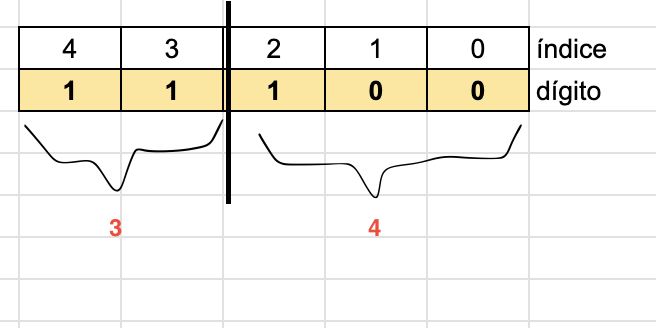
\includegraphics[width=0.6\textwidth]{Figuras/agrupamento_de2_para8.png}
        \label{fig-agrupamento2-8}
    \end{figure}
    %-------------------Figure---------------------


    \begin{align*}
        11100_2 & = 1\times2^4 + 1\times2^3 + 1\times2^2 + 0\times2^1 + 0\times2^0 \\
                & = 2^4 + 2^3 + 2^2                                                \\
                & = (2^1 + 2^0) \times 2^3 + 2^2                                   \\
                & = (2 + 1) \times 8 + 4                                           \\
                & = 3 \times 8 + 4                                                 \\
                & = 3 \times 8^1 + 4 \times 8^0                                    \\
                & = 34_8
    \end{align*}



\end{frame}

\begin{frame}{Conversão: Base 16 para Base 2}

    Como $16 = 2^4$, cada símbolo da representação hexadecimal corresponde a um grupo de \textbf{4 bits}.



    \textbf{Procedimento:}
    \begin{itemize}
        \item Cada dígito hexadecimal deve ser expandido em sua representação binária de 4 bits.
        \item \textbf{Atenção:} Deve-se usar zeros à esquerda para completar os 4 bits em valores menores que $8$ (ex: $1_{16} \rightarrow 0001_2$).
    \end{itemize}
\end{frame}

\begin{frame}{Exemplo Detalhado: $1C_{16}$}
    Vamos decompor o número $1C_{16}$ utilizando potências de 2:

    \begin{itemize}
        \item $1C_{16} = C \times 16^0 + 1 \times 16^1$
        \item $1C_{16} = 12 \times 16^0 + 1 \times 16^1$
        \item $1C_{16} = 12 \times (2^4)^0 + 1 \times (2^4)^1$
        \item $1C_{16} = 12 \times 2^0 + 1 \times 2^4$
    \end{itemize}

    Sabendo que $C_{16} = 12_{10} = 1100_2$ (ou $2^3 + 2^2$), substituímos:

    \begin{itemize}
        \item $1C_{16} = (2^3 + 2^2) \times 2^0 + 1 \times 2^4$
        \item $1C_{16} = 2^3 + 2^2 + 2^4$
        \item $1C_{16} = 11100_2$
    \end{itemize}
\end{frame}

\begin{frame}{Tabela de Conversão: Hexadecimal $\rightarrow$ Binário}
    \begin{itemize}
        \item Como $16 = 2^4$, cada dígito hexadecimal corresponde a \textbf{4 bits} na representação binária.
        \item Substituímos cada símbolo pelo seu equivalente binário de 4 dígitos.
    \end{itemize}

    \begin{table}[]
        \centering
        \small
        \begin{tabular}{|c|c||c|c|}
            \hline
            \textbf{Hex} & \textbf{4 bits Binário} & \textbf{Hex} & \textbf{4 bits Binário} \\ \hline
            $0_{16}$     & $0000_2$                & $8_{16}$     & $1000_2$                \\ \hline
            $1_{16}$     & $0001_2$                & $9_{16}$     & $1001_2$                \\ \hline
            $2_{16}$     & $0010_2$                & $A_{16}$     & $1010_2$                \\ \hline
            $3_{16}$     & $0011_2$                & $B_{16}$     & $1011_2$                \\ \hline
            $4_{16}$     & $0100_2$                & $C_{16}$     & $1100_2$                \\ \hline
            $5_{16}$     & $0101_2$                & $D_{16}$     & $1101_2$                \\ \hline
            $6_{16}$     & $0110_2$                & $E_{16}$     & $1110_2$                \\ \hline
            $7_{16}$     & $0111_2$                & $F_{16}$     & $1111_2$                \\ \hline
        \end{tabular}
    \end{table}
\end{frame}

\begin{frame}{Método Simplificado (Mapeamento Direto)}
    A forma mais rápida é a concatenação de grupos de 4 bits:

    \begin{table}
        \centering
        \begin{tabular}{|c|c|}
            \hline
            \textbf{Hexadecimal} & \textbf{Binário (4 bits)} \\ \hline
            $1_{16}$             & $0001_2$                  \\ \hline
            $C_{16}$             & $1100_2$                  \\ \hline
        \end{tabular}
    \end{table}

    \vspace{0.3cm}
    \textbf{Resultado:}
    \begin{displaymath}
        1C_{16} = \underbrace{0001}_{1} \underbrace{1100}_{C} = 00011100_2
    \end{displaymath}

    \vspace{0.3cm}
    Removendo os zeros à esquerda:
    $$1C_{16} = 11100_2$$
\end{frame}

\begin{frame}{Exercício}
    Converta \textbf{sem passar para a base 10} os seguintes números da base 8 para a base 2:


    \begin{enumerate}[a)]
        \item $20_8$
        \item $7_8$
        \item $407_8$
        \item $2022_8$

    \end{enumerate}

    Converta \textbf{sem passar para a base 10} os seguintes números da base 16 para a base 2:
    \begin{enumerate}[a)]
        \item  $20_{16}$
        \item  $7_{16}$
        \item  $407_{16}$
        \item  $2022_{16}$
        \item  $ABCD_{16}$
    \end{enumerate}
\end{frame}

\begin{frame}{Exercício -- Gabarito}
    Converta \textbf{sem passar para a base 10} os seguintes números da base 8 para a base 2 \textcolor{red}{grupos de 3 bits}:

    \begin{enumerate}[a)]
        % \hfill empurra o texto para a direita, \textcolor{red} muda a cor
        \item $20_8$ = \textcolor{red}{$010\,000_2 = 10000_2$}
        \item $7_8$ = \textcolor{red}{$111_2$}
        \item $407_8$ = \textcolor{red}{$100\,000\,111_2$}
        \item $2022_8$ = \textcolor{red}{$010\,000\,010\,010_2 = 10000010010_2$}
    \end{enumerate}

    \vspace{0.3cm} % Espaçamento entre os blocos

    Converta \textbf{sem passar para a base 10} os seguintes números da base 16 para a base 2 \textcolor{red}{grupos de 4 bits}:
    \begin{enumerate}[a)]
        \item $20_{16}$ = \textcolor{red}{$0010\,0000_2 = 100000_2$}
        \item $7_{16}$ = \textcolor{red}{$0111_2 = 111_2$}
        \item $407_{16}$ = \textcolor{red}{$0100\,0000\,0111_2 = 10000000111_2$}
        \item $2022_{16}$ = \textcolor{red}{$0010\,0000\,0010\,0010_2 = 10000000100010_2$}
        \item $ABCD_{16}$ = \textcolor{red}{$1010\,1011\,1100\,1101_2$}
    \end{enumerate}
\end{frame}

